\documentclass[a4paper]{article}
\usepackage[utf8x]{inputenc}
\usepackage[T1,T2A]{fontenc}
\usepackage[russian]{babel}
\usepackage{hyperref}
\usepackage{indentfirst} % включить отступ у первого абзаца
\usepackage{listings}
\lstset{inputpath=../listings}
\usepackage{color}
\usepackage{here} 
\usepackage{graphicx}
\graphicspath{{pics/}}

\usepackage{caption}
\renewcommand{\lstlistingname}{Листинг}

\usepackage{listings}
\lstdefinestyle{base_listing}{ %
extendedchars=\true,
basicstyle=\footnotesize,       % the size of the fonts that are used for the code
numbers=left,                   % where to put the line-numbers
numberstyle=\footnotesize,      % the size of the fonts that are used for the line-numbers
stepnumber=1,                   % the step between two line-numbers. If it is 1 each line will be numbered
numbersep=5pt,                  % how far the line-numbers are from the code
backgroundcolor=\color{white},  % choose the background color. You must add \usepackage{color}
showspaces=false,               % show spaces adding particular underscores
showstringspaces=false,         % underline spaces within strings
showtabs=false,                 % show tabs within strings adding particular underscores
frame=single,           % adds a frame around the code
tabsize=2,          % sets default tabsize to 2 spaces
captionpos=b,           % sets the caption-position to bottom
breaklines=true,        % sets automatic line breaking
breakatwhitespace=false,    % sets if automatic breaks should only happen at whitespace
escapeinside={\%*}{*)},          % if you want to add a comment within your code
postbreak=\raisebox{0ex}[0ex][0ex]{\ensuremath{\color{red}\hookrightarrow\space}},
keepspaces = true
}

\lstdefinestyle{crs_bash}{
  style    = {base_listing},
  language = {bash}
}

\lstdefinestyle{crs_cpp}{
  style    = {base_listing},
  language = {C++}
}

\usepackage[left=2.5cm, top=2cm, right=2cm, bottom=2cm, nohead]{geometry}

\begin{document}
\begin{titlepage} % начало титульной страницы

\begin{center} % включить выравнивание по центру

\large Санкт-Петербургский Политехнический Университет Петра Великого\\
\large Институт компьютерных наук и технологий \\
\large Кафедра компьютерных систем и программных технологий\\[6cm]
% название института, затем отступ 4,5см

\huge Операционные системы и среды\\[0.5cm]
\large Отчет по лабораторной работе №3\\[0.1cm]
\large Процессы в UNIX-системах\\[5cm]
\end{center}

\begin{flushright}
\begin{minipage}{0.5\textwidth}
\begin{flushright}
\textbf{Работу выполнил:}

Петров Владислав

{Группа:} 43501/4\\


\textbf{Преподаватель:} 

Душутина Елена Владимировна
\end{flushright}
\end{minipage} % конец врезки
\end{flushright} % конец выравнивания по левому краю

\vfill % заполнить всё доступное ниже пространство

\begin{center}

\large Санкт-Петербург\\
\large \the\year % вывести дату

\end{center} % закончить выравнивание по центру

\thispagestyle{empty} % не нумеровать страницу
\end{titlepage} % конец титульной страницы

\vfill % заполнить всё доступное ниже пространство


\section{Цель работы}
	Изучить способы управления процессами и потоками в ОС семейства Windows.
	
\section{Ход работы}
\subsection{Создание процессов}
	Рассмотрим создание одного процесса другим посредством функции WinAPI \textbf{CreateProcess}. При создании исполнительная система выполняет работу по организации окружения (среды исполнения процесса) и предоставлению необходимых ему ресурсов. Она выделяет новое адресное пространство и иные ресурсы для процесса, а также создает для него новый базовый поток. Когда новый процесс будет создан, старый процесс будет продолжать исполняться, используя старое адресное пространство, а новый будет выполняться в новом адресном пространстве с новым базовым потоком. После того, как исполнительная система создала новый процесс, она возвращает его описатель, а также описатель его базового потока.
	Синтаксис команды \textbf{CreateProcess}:
	\begin{lstlisting}[style=crs_cpp]
BOOL CreateProcess( LPCTSTR lpApplicationName, // имя исполняемого модуля
					LPTSTR lpCommandLine, // командная строка
					LPSECURITY_ATTRIBUTES lpProcessAttributes, // атрибуты безопасности процесса 
					LPSECURITY_ATTRIBUTES lpThreadAttributes, // атрибуты безопасности потока 
					BOOL bInheritHandeles, // флаг наследования описателя 					
					DWORD dwCreationFlags, // флаги создания
					LPVOID lpEnvironment, // новый блок окружения 
					LPCTSTR lpCurrentDirectory, // имя текущей директории 
					LPSTARTUPINFO lpStartupInfo, // STARTUPINFO
					LPPROCESS_INFORMATION lpProcessInformation // PROCESS_INFORMATION 
					)
	\end{lstlisting}
	
	\textbf{CreateProcess()} отводит место под объекты процесс и поток и возвращает значения их описателей (индексы в таблице) в структуре\\ \texttt{PROCESS\_INFORMATION}.
	
	Освободить выделенное место можно вызовом \textbf{CloseHandle}. При этом выполнение этого вызова не обязательно приведет к завершению процесса (только исчезнет ссылка на объект внутри вызвавшего процесса).
	
	\textbf{CreateProcess()} возвращает ноль, если создание процесса прошло успешно.
	
	\textbf{Задание} Программа после запуска должна создать новый процесс, с помощью функции CreateProcess. В новом процессе необходимо запустить любое приложение (например, notepad.exe или calc.exe). Для контроля можно вывести идентификаторы созданного процесса и потока, а затем завершить основную программу.
	
	Исходный код программы (task\_1.cpp), создающей процесс для запуска приложения notepad.exe и открытия блокнота с файлом без имени:
	\lstinputlisting[style=crs_cpp]{task_1.cpp}
	
	Параметр lpApplicationName установлен NULL. В этом случае, имя модуля должно быть в строке lpCommandLine.
	
	В данном случае будем использовать значения по умолчанию для атрибутов безопасности процесса и потока --– NULL (параметры lpProcessAttributes и lpThreadAttributes ) и FALSE для флага наследования (bInheritHandles).
	
	Для создания нового процесса (child) с высоким приоритетом в его собственном окне используем --- \texttt{HIGH\_PRIORITY\_CLASS | CREATE\_NEW\_CONSOLE}.
	
	Параметр lpEnvironment используется для передачи нового блока переменных окружения порожденному процессу-потомку (child). Если указано NULL –-- то потомок использует то же окружение, что и родитель.
Параметр lpCurrentDirectory установлен в (NULL). Это означает, что новый процесс создается с тем же самым текущим диском и каталогом, что и вызывающий процесс.
	
	В структуре startupInfo устанавливаются оконный режим терминала, рабочий стол, стандартные дескрипторы и внешний вид главного окна для нового процесса.
	
	В структуре processInfo хранятся: описатель вновь созданного процесса (hProcess), описатель его базового потока (hThread), глобальный идентификатор процесса (dwProcessId), глобальный идентификатор потока (dwThreadId).
	
	Результат работы программы приведен на рисунке \ref{img:task1}.
	\begin{figure}[h]
		\center{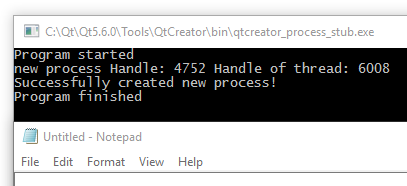
\includegraphics[scale=0.75]{task1}}
		\caption{Результат работы программы task\_1.cpp}
		\label{img:task1}
	\end{figure}
	
	\textbf{Задание} Программа, получает имя конфигурационного файла из командной строки, открывает конфигурационный файл, читает строки и создает для запуска каждой команды отдельный процесс.
	
	С целью упрощения кода сначала имя командного файла зададим прямо в программе и представим текст программы без обработки возможных ошибок. Создаем конфигурационный файл с именем "temp.txt" при помощи текстового редактора(например, notepad) и располагаем его в корневом каталоге диска С. Далее записываем в файл следующие строки:
	\begin{lstlisting}[style=crs_cpp]
C:\Windows\System32\NOTEPAD.EXE
C:\Windows\System32\CALC.EXE
	\end{lstlisting}
	
	Исходный код программы task\_2.cpp:	
	\lstinputlisting[style=crs_cpp]{task_2.cpp}
	
	Результат работы программы приведен на рисунке \ref{img:task2}.
	\begin{figure}[h!]
		\center{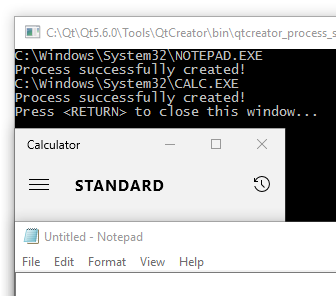
\includegraphics[scale=0.75]{task2}}
		\caption{Результат работы программы task\_2.cpp}
		\label{img:task2}
	\end{figure}
	
	Доработаем программу. Пусть программа получает имя конфигурационного файла в качестве аргумента из командной строки, открывает его с помощью fopen(), читает построчно функцией fgetws(). После прочтения каждой строки, если она не пуста, создается процесс, в командную строку которого пишется прочитанная строка. Если создать процесс не удалось, программа пробует читать конфигурационный файл дальше.
	
		Исходный код программы task\_2\_changed.cpp:
	\lstinputlisting[style=crs_cpp]{task_2_changed.cpp}
	
	Результат работы программы приведен на рисунке \ref{img:task2changed}.
	\begin{figure}[h!]
		\center{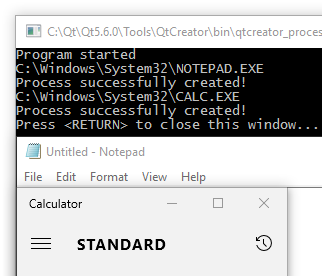
\includegraphics[scale=0.75]{task2changed}}
		\caption{Результат работы программы task\_2\_changed.cpp}
		\label{img:task2changed}
	\end{figure}
	
	Вызов процессов производится здесь без синхронизации. Процесс-родитель не дожидается создания процессов-потомков, а им после создания необходимо разбирать строку аргументов. Когда передается один неверный аргумент, процесс не создается (т.к. сразу проверяется наличие исполняемого файла с указанным именем). <<Error 2>> соответствует ошибка <<Файл не найден>>. При передаче в commandLine процесса строки из нескольких слов процесс все равно создается (даже если аргументы не верны), но быстро завершается. При этом созданные процессы связаны с консолью процесса-родителя (аргумент DwCreationFlags в вызове CreateProcess равен 0).
	
	\subsection{Создание потоков}	
	Cоздание потоков посредством функции WinAPI \textbf{CreateThread}:
	\begin{lstlisting}[style=crs_cpp]
HANDLE CreateThread( 
	LPSECURITY_ATTRIBUTES lpsa, //дескриптор защиты 
	DWORD dwStackSize, // начальный размер стека 
	LPTHREAD_START_ROUTINE lpStartAddr, //функция потока 
	LPVOID lpThreadParm, //параметр потока 
	DWORD dwCreationFlags, //опции создания 
	LPDWORD lpThreadId //идентификатор потока 
	)	
	\end{lstlisting}
	
	Если функция выполнилась успешно, то вернется описатель потока, если нет, вернется NULL.
	
	\textbf{Задание} Программа должна создавать два потока, выводящих в бесконечном цикле <<1>> и <<2>> соответственно. После создания дополнительных потоков, поток-родитель завершается.
	
	В данной программе после создания потоков, главный поток завершается, способов завершения может быть два: с помощью return и с помощью вызова функции ExitThread.
	
	Исходный код программы task\_3.cpp:
	\lstinputlisting[style=crs_cpp]{task_3.cpp}
	
	Результат работы программы приведен на рисунках \ref{img:task3_1} -- \ref{img:task3_2}.
	\begin{figure}[h!]
		\center{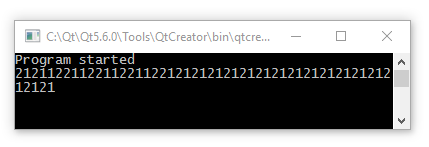
\includegraphics[scale=0.75]{task3_1}}
		\caption{Результат работы программы task3.cpp с завершением при помощи ExitThread(0)}
		\label{img:task3_1}
	\end{figure}
	
	\begin{figure}[h!]
		\center{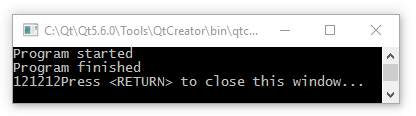
\includegraphics[scale=0.75]{task3_2}}
		\caption{Результат работы программы task3.cpp с завершением при помощи return}
		\label{img:task3_2}
	\end{figure}
	
	Очевидно, что в первом случае завершился только главный поток, а процесс – нет, а во втором - произошло завершение всего процесса.
	
	Аналогичные результаты будут, если основной поток после создания потомков выполнит функцию \textbf{Sleep()} с неопределенным временем ожидания.
	
	Функция \textbf{Sleep()} позволяет потоку отказаться от использования процессора и перейти из состояния выполнения в состояние ожидания, которое будет длиться в течение заданного промежутка времени. Например, выполнение задачи потоком может продолжаться в течение некоторого периода времени, после чего поток приостанавливается. По истечении периода ожидания планировщик вновь переводит поток в состояние готовности.
	
	\textbf{Задание} Программа должна получать 2 параметра --– количество создаваемых потоков и время жизни всего приложения. С интервалом в 1 сек каждый рабочий поток выводит о себе информацию и отслеживает состояние переменной, которая устанавливается в заданное значение по истечении времени жизни процесса.
	
	Возможны различные варианты решения данной задачи. Например, для подсчета времени можно использовать поток-координатор, вычисляющий момент завершения периода жизни с помощью функции \textbf{getTickCount()}, (сравнивая разницу текущего и стартового времени с заданным периодом жизни) или с помощью функции получения системного времени \textbf{GetSystemTime (\&now)}. Другой способ (более рациональный) --- использование таймера ожидания (Waitable Timer).
Рассмотрим вариант на основе таймера ожидания.

	Таймеры ожидания(waitable timers) – это объекты ядра, которые самостоятельно переходят в свободное состояние в определенное время или через регулярные промежутки времени. Чтобы создать ожидаемый таймер, достаточно вызвать функцию \textbf{CreateWaitableTimer()}. Объекты <<ожидаемый таймер>> всегда создаются в занятом состоянии. Чтобы сообщить таймеру, в какой момент он должен перейти в свободное состояние, необходимо вызвать функцию \textbf{SetWaitableTimer}.
	
	Исходный код программы task\_4.cpp:
	\lstinputlisting[style=crs_cpp]{task_4.cpp}
	
	Результат работы программы приведен на рисунке \ref{img:task4}
	\begin{figure}[h!]
		\center{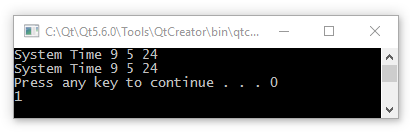
\includegraphics[scale=0.75]{task4}}
		\caption{Результат работы программы task4.cpp}
		\label{img:task4}
	\end{figure}
	
	\subsection{Функции управления приоритетами процессов и потоков}
	Windows поддерживает шесть классов приоритета процесса: idle (простаивающий), below normal (ниже обычного), normal (обычный), above normal (выше обычного), high (высокий), real-time (реального времени).
	
	Кроме того, Windows поддерживает семь относительных приоритетов потока: idle (простаивающий), lowest (низший), below normal (ниже обычного), normal (обычный), above normal (выше обычного), highest (высший) и time-critical (критичный по времени).
	
	Относительный приоритет потока принимает значение от 0 (самый низкий) до 31 (самый высокий), но программист работает не с численными значениями, а с так называемыми <<константными>>. Это обеспечивает определенную гибкость и независимость при изменении алгоритмов планирования, а они меняются практически с каждой новой версией ОС, а с ними, соответственно, могут измениться и соотношения приоритетов.
Уровень приоритета формируется самой системой, исходя из класса приоритета процесса и относительного приоритета потока.

	Динамическое повышение приоритета предназначено для оптимизации общей пропускной способности и реактивности системы, при этом выигрывает не каждое приложение в отдельности, а система в целом.
Windows может динамически повышать значение текущего приоритета потока в одном из следующих случаев:
	\begin{enumerate}
	\item после завершения операции ввода/вывода;
	\item по окончании ожидания на каком-либо объекте исполнительной системы;
	\item при нехватке процессорного времени и инверсии приоритетов.	
	\end{enumerate}
	
	Система повышает приоритет только тех потоков, базовый приоритет которых попадает в область динамического приоритета (dynamic priority range), т.е. находится в пределах 1-15. ОС не допускает динамического повышения приоритета прикладного потока до уровней реального времени.
	
	Системные функции обслуживаются с приоритетами реального времени. ОС никогда не меняет приоритет потоков с уровнями реального времени (от 16 до 31). Это ограничение позволяет сохранять целостность системы и обеспечивает необходимый уровень безопасности.
	
	\textbf{Задание} Подготовить программу, в которой у каждого из потоков свой приоритет отличный от других. Все они выполняют одинаковую работу, например, увеличивают каждый свой счетчик. Накопленное значение счетчика, таким образом, отражает относительное суммарное время выполнения потока.
	
	Предполагаем, так как приоритеты различны, то и время, отведенное на работу потокам различно (квант времени, выделяемый потокам, одинаков).
	
	Исходный код программы task\_5.cpp:
	\lstinputlisting[style=crs_cpp]{task_5.cpp}
	
	Результат работы программы приведен на рисунке \ref{img:task5}
	\begin{figure}[h!]
		\center{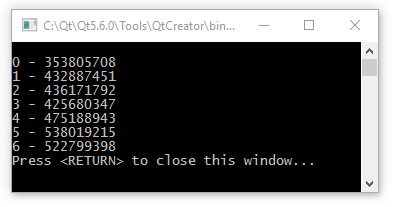
\includegraphics[scale=0.75]{task5}}
		\caption{Результат работы программы task\_5.cpp}
		\label{img:task5}
	\end{figure}
	
	Слева --- номер класса приоритета от низшего к высшему, а справа --- значение счетчика, накопленное за все кванты, предоставленные потоку до истечения таймера. Очевидно, что потокам, у которых приоритет ниже, выделяется меньшее количество квантов времени для выполнения, и поэтому их счетчики соответственно меньше. При каждом запуске экспериментальные данные получаются различными, но пропорциональное соотношение между счетчиками потоков примерно сохраняется.\\
	
\subsection{Управление классом приоритетов процесса}
	Усложним задачу и дополним ее возможностью управлять классом приоритетов процесса. Программа по-прежнему создает 7 дополнительных потоков, со всеми возможными вариантами приоритета. Теперь в начале работы можно изменить класс приоритета процесса в целом. Каждый рабочий процесс выполняет увеличение связанного с ним счетчика (здесь типа int). После увеличения счетчика, поток отдает оставшуюся часть кванта времени остальным, с помощью вызова функции Sleep с параметром 0. Через заданное время рабочие потоки завершаются, а основной поток выводит результаты их работы в новом формате. Окончание работы происходит по сигналу от таймера. Заложена возможность задания произвольного количества потоков и времени жизни, отсчитываемого таймером.
			
	Исходный код программы task\_6.cpp:
	\lstinputlisting[style=crs_cpp]{task_6.cpp}
	
	Результат работы программы приведен на рисунках \ref{img:task6} --\ref{img:task6_2}.
	\begin{figure}[h!]
		\center{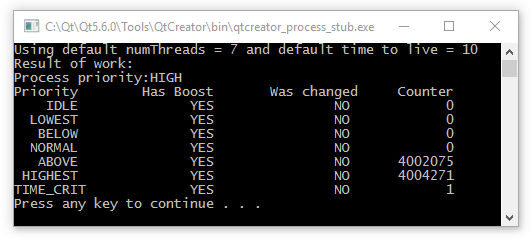
\includegraphics[scale=0.75]{task6}}
		\caption{Результат работы программы task6.cpp на однопроцессорной системе}
		\label{img:task6}
	\end{figure}
	
	\begin{figure}[h!]
		\center{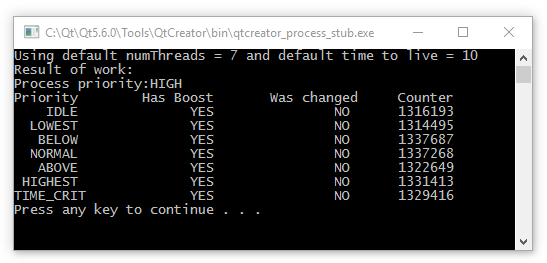
\includegraphics[scale=0.75]{task6_2}}
		\caption{Результат работы программы task6.cpp при использовании нескольких процессоров}
		\label{img:task6_2}
	\end{figure}
	
\subsection{Функций динамического управления приоритетами}
	\textbf{Задача} Анализ поведения системных функций динамического управления приоритетами процессов и потоков.
	
	С помощью программы определим, назначается ли динамическое изменение приоритетов по умолчанию, на все ли потоки воздействует функция SetProcessPriorityBoost(), возможно ли разрешение отдельному потоку в процессе динамически изменять приоритет, если для процесса это запрещено.
	
	Исходный код программы task\_7.cpp:
	\lstinputlisting[style=crs_cpp]{task_7.cpp}
	
	Результат работы программы приведен на рисунке \ref{img:task7}.
	\begin{figure}[h!]
		\center{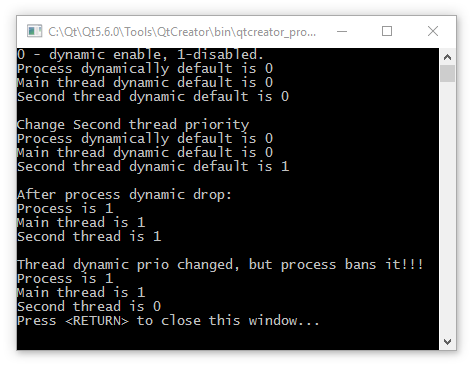
\includegraphics[scale=0.75]{task7}}
		\caption{Результат работы программы task7.cpp}
		\label{img:task7}
	\end{figure}
	Из листингов видно, что по умолчанию для  процессов и потоков динамическое изменение приоритетов разрешено. Потом для второго потока было запрещено изменение динамического приоритета с помощью функции SetThreadPriorityBoost. Если запретить динамическое изменение приоритетов для процесса (SetProcessPriorityBoost), то изменение также будет запрещено и для всех потоков. Разрешение отдельному потоку в процессе динамически изменять приоритет возможно, если для процесса это запрещено.
	\subsection{Самостоятельные задания}
	Исследуйте результаты работы программы task5.cpp и task6.cpp в зависимости от того, какой приоритет назначается базовому потоку; своими экспериментальными данными заполните таблицу с точным указанием для какой ОС и на каком отладочном комплексе проводились измерения.
	
	Исследование проводилось на ОС Windows 10.
	
	\begin{table}[h!]
		\small
		\begin{tabular}{|c|c|c|c|c|c|c|c|}
		\hline 
		& idle & below normal & normal & above normal & highest & time critical \\ 
		\hline 
		idle & 384889470 & 338750935 & 370475172 & 397654353 & 375165721 & 367254998   \\ 
		\hline 
		lowest & 442457983 & 409933756 & 438973987 & 460370700 & 388419286 & 449369600 \\ 
		\hline 
		below normal & 453232814 & 447691472 & 454739216 & 468485519 & 509029435 & 498882038 \\ 
		\hline 
		normal & 471224827 & 499423558 & 463177844 & 463073975 & 578848964 & 481554700 \\ 
		\hline 
		above normal & 461201143 & 441116575 & 468579495 & 421960961 & 364916750 & 468927130 \\ 
		\hline 
		highest & 458434552 & 479824772 & 502420426 & 468361146 & 414371949 & 463562081\\ 
		\hline 
		time critical & 517431059 & 494322870 & 479882926 & 493014328 & 491354487 & 475320493\\ 
		\hline 
		\end{tabular} 
		\caption{Исследование программы task\_5.cpp для различных значений приоритета базового потока}
	\end{table}
	
	По результатам исследования можно сказать, что пропорциональное соотношение между счетчиками потоков примерно сохраняется при любых значениях приоритета базового потока. Однако, судя по результатам, значение приоритета базового потока несильно влияет на время, выделяемое процессу. Возможно, это происходит из-за того, что выполнение программы прерывается другими программами, имеющими больший приоритет.
	
	Модифицируйте программу task5.cpp для заполнения таблицы 2 текущими данными вашего эксперимента. Сделайте выводы.
	\begin{figure}[h!]
		\center{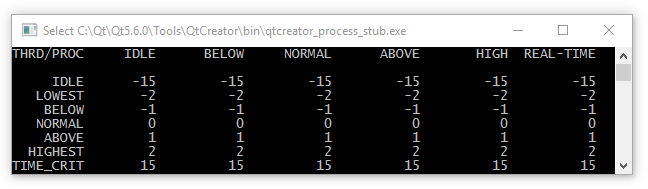
\includegraphics[scale=0.75]{task9}}
		\caption{Примерная зависимость уровня приоритета потока}
		\label{img:prio_dep}
	\end{figure}
	По результатам исследования можно предположить, что в данной системе приоритет потока не зависит от класса потока.\\
	
	С помощью утилиты CPU Stress test, которая позволяет нагружать систему, и утилиты мониторинга ProcessExplorer() было зафиксировано динамическое изменение приоритетов. 
	\begin{figure}[h!]
		\center{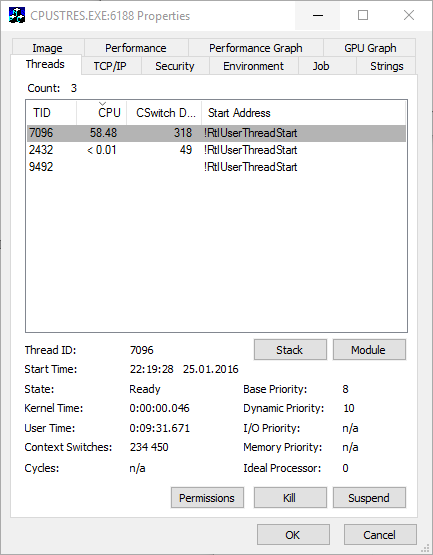
\includegraphics[scale=0.75]{task10}}
		\caption{Динамический приоритет потока в программе CPU Stress}
		\label{img:dyn_cha}
	\end{figure}
	В разгруженной системе выполнение программ task5 task6 происходит слишком быстро, мы не успеваем зафиксировать их появления в утилите мониторинга. После запуска утилиты CPU Stress test время работы программ значительно увеличивается.
	\begin{figure}[h!]
		\center{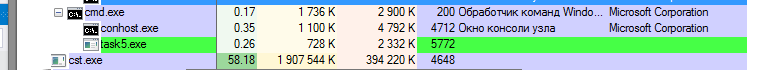
\includegraphics[scale=0.75]{cpu_test}}
		\caption{Утилита мониторинга нагруженной системы}
		\label{img:cpu_test}
	\end{figure}
	
	По рисунку видно, что большую часть процессорного времени занимает CPU Stress test (процесс cst.exe). Нашей программе выделяется очень мало процессорного времени.\\

	 Создайте программу, демонстрирующую возможность наследования
	 \begin{itemize}
\item дескриптора порождающего процесса,
\item дескрипторов открытых файлов,
	 \end{itemize}
Для выполнения этого задания следует учесть, что по умолчанию наследование в Windows отключено и для возможности наследования, необходимо:
	 \begin{enumerate}
\item  разрешить процессу-потомку наследовать дескрипторы,
\item  сделать дескрипторы наследуемыми
	\end{enumerate}
	Напишем программу, которая создает файл, в который будут записываться данные родительским и дочерним процессом.
	Программа родитель:
	\lstinputlisting[style=crs_cpp]{writer_parent.cpp}
	
	Программа ребёнок:
	\lstinputlisting[style=crs_cpp]{writer_child.cpp}
	
	Содержимое файла, созданного в текущей директории представлено на рисунке \ref{img:fd}. Наличие вывода обеих программ говорит об успешной передаче дескрипторов открытых файлов
	
	\begin{figure}[h!]
		\center{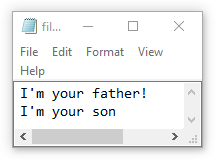
\includegraphics[scale=0.75]{task11}}
		\caption{Утилита мониторинга нагруженной системы}
		\label{img:fd}
	\end{figure}

\section{Вывод}
	В данной работе было изучено управление процессами и потоками в ОС Windows.
	
	В отличие от систем Unix, в системе Windows первичными являются потоки, а не процессы. Поток --– системный объект операционной системы, реально выполняющийся в процессоре. Процесс --– абстрактная структура, определяющая единое адресное пространство и контекст одного или нескольких взаимосвязанных потоков. При создании любого процесса всегда создается первичный поток.
	
	Функции управления процессами и потоками имеют большое количество аргументов, причем некоторые из них достаточно сложные и информационно емкие. Это позволяет производить гибкую настройку параметров создаваемых процессов, однако при первом ознакомлении оказывается достаточно сложным.
	
	
	Важным аспектом приоритетов является связь приоритета процесса с приоритетом потока и не только ручное регулирование приоритета, а так же и динамическое, осуществляемое операционной системой с целью достижения большей общей производительности.

\end{document}

